% Copyright (C) 2005-2015 Airbus - EDF - IMACS - Phimeca
% Permission is granted to copy, distribute and/or modify this document
% under the terms of the GNU Free Documentation License, Version 1.2
% or any later version published by the Free Software Foundation;
% with no Invariant Sections, no Front-Cover Texts, and no Back-Cover
% Texts.  A copy of the license is included in the section entitled "GNU
% Free Documentation License".
\renewcommand{\etapemethodo}{C}
\renewcommand{\nomfichier}{docref_C11_ExperimentPlanes}
\renewcommand{\titrefiche}{Design of Experiments}

\Header

\MathematicalDescription
    {
      \underline{\textbf{Goal}} \vspace{2mm}

      The method is used in the following context: $\vect{x}= \left( x^1,\ldots,x^{n_X} \right)$ is a vector of input parameters. We want to determine a particular set of values of $\vect{x}$ according to a particular design of experiments .
      \vspace*{2mm}

      \underline{\textbf{Principle}}
      \vspace{2mm}

      Different types of design of experiments can be determined:
      \begin{itemize}
      \item some \emph{stratified} patterns: axial, composite, factorial or box patterns,
      \item some \emph{weighted} patterns that we can split into different categories: the random patterns, the low discrepancy sequences and the Gauss product.
      \end{itemize}

      \vspace*{2mm}

      {\bf Stratified design of experiments }\\

      All stratified design of experiments are defined from the data of a center point and some discretization levels. OpenTURNS proposes the same number of levels for each direction: let us denote by $n_{level}$ that discretization number.\\

      The axial pattern contains points only along the axes. It is not convenient to model interactions between variables. The pattern is obtained by discretizing each direction according to specified levels, symmetrically with respect to the center of the design of experiments . The number of points generated is $1 + 2dn_{level}$.\\

      The factorial pattern contains points only on diagonals. It is not convenient to model influences of single input variables. The pattern is obtained by discretizing each principal diagonal according to the specified levels, symmetrically with respect to the center of the design of experiments . The number of points generated is $1 + 2^dn_{level}$.\\

      The composite pattern is the union of both previous ones. The number of points generated is $1 + 2dn_{level} + 2^dn_{level}$.\\

      The box pattern is a simple regular discretization of a pavement around the center of the design of experiments , with the number of intermediate points specified for each direction (denoted $n_{level}(direction \, \, i)$). The number of points generated is $\displaystyle \prod_{i=1}^{d} (2+n_{level}(direction \, \, i))$.\\

      The following figures illustrates the different patterns obtained.

      \newpage
      \begin{center}
        \begin{tabular}{cc}
          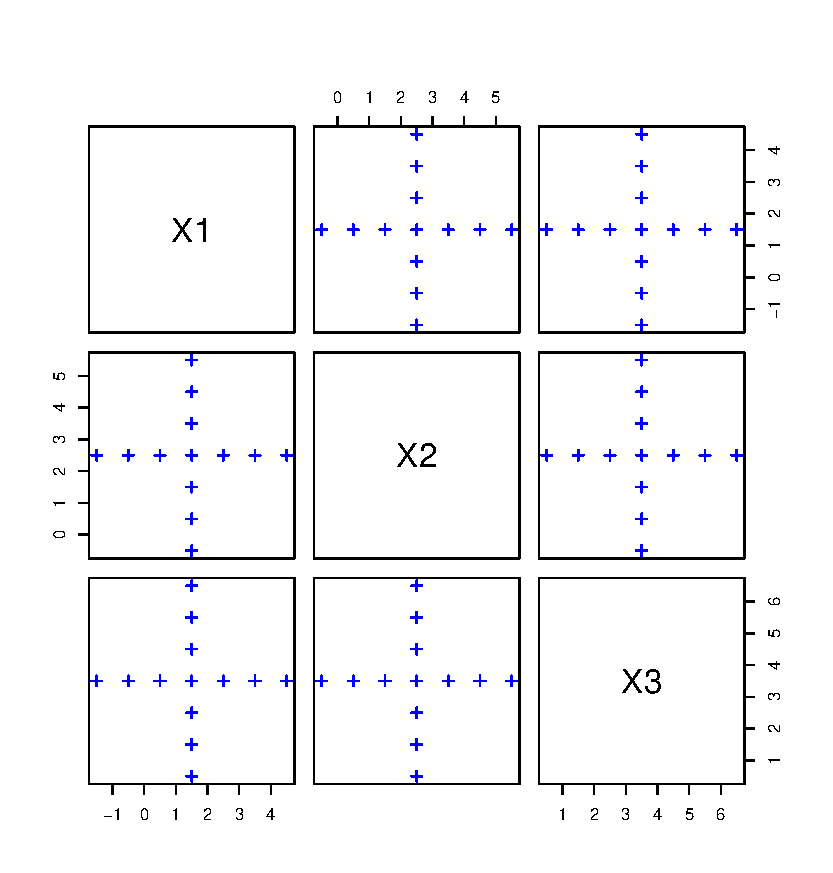
\includegraphics[width=8cm]{Figures/Axial_DOE.pdf} & 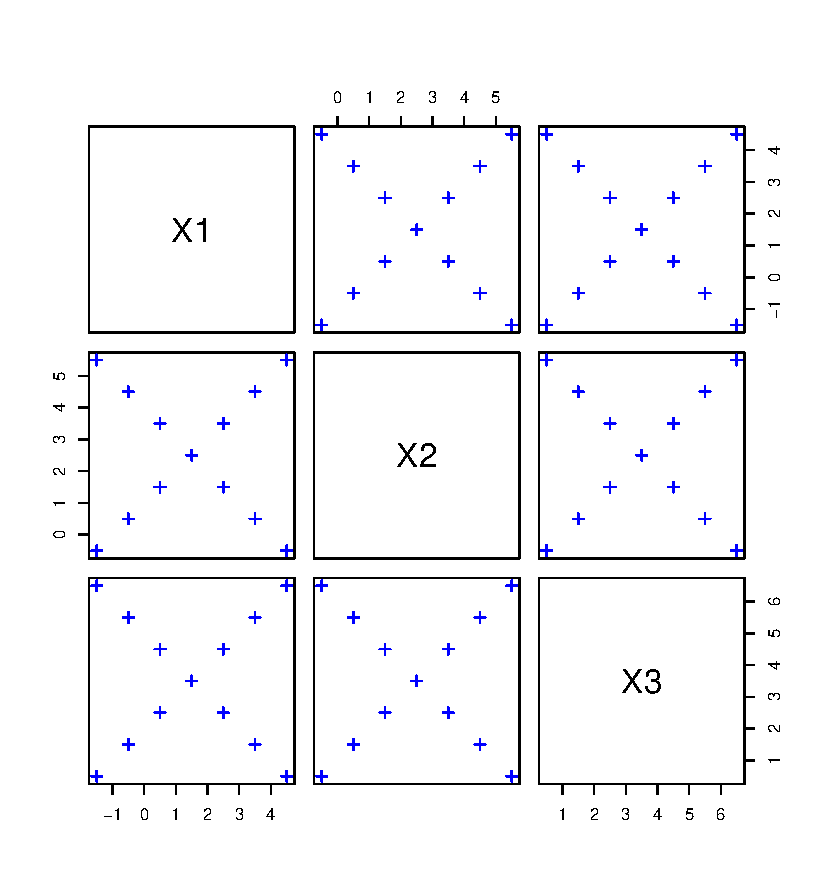
\includegraphics[width=8cm]{Figures/Factorial_DOE.pdf}\\
          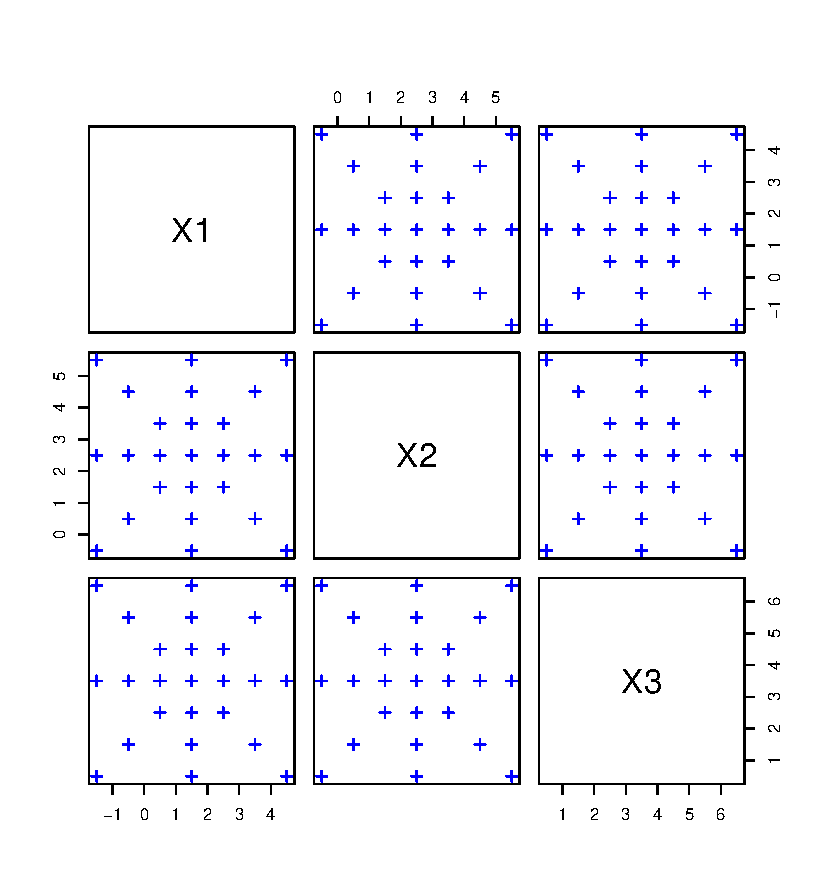
\includegraphics[width=8cm]{Figures/Composite_DOE.pdf} & 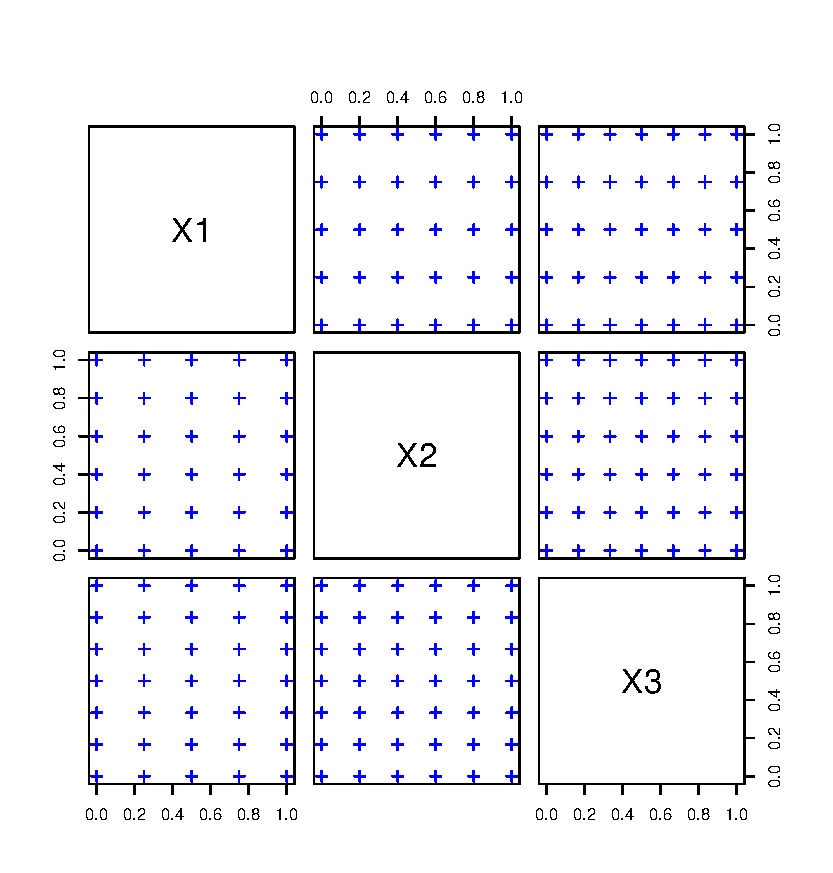
\includegraphics[width=8cm]{Figures/Box_DOE.pdf}
        \end{tabular}
      \end{center}

      \vspace*{2mm}

      {\bf Weighted design of experiments }\\

      The first category is the {\itshape random patterns}, where the set of input data is generated from the joint distribution of the input random vector, according to the Monte Carlo sampling technique or the LHS one (refer to \otref{docref_C321_MonteCarloStd}{Monte Carlo Simulation} and \otref{docref_C322_LHS}{Latin Hypercube Sampling}).\\
      Care: the LHS sampling method requires the independence of the input random variables.\\

      The second category is the {\itshape low discrepancy sequences} (refer to \otref{docref_C_LowDiscrepancySequence}{Low Discrepancy Sequence}). OpenTURNS proposes the Faure, Halton, Haselgrove, Reverse Halton and Sobol sequences.\\


      The third category is the {\itshape Gauss product} which is the set of points which components are the respective Gauss set (i.e. the roots of the orthogonal polynomials with respect to the univariate distribution).

      \newpage
      \begin{center}
        \begin{tabular}{cc}
          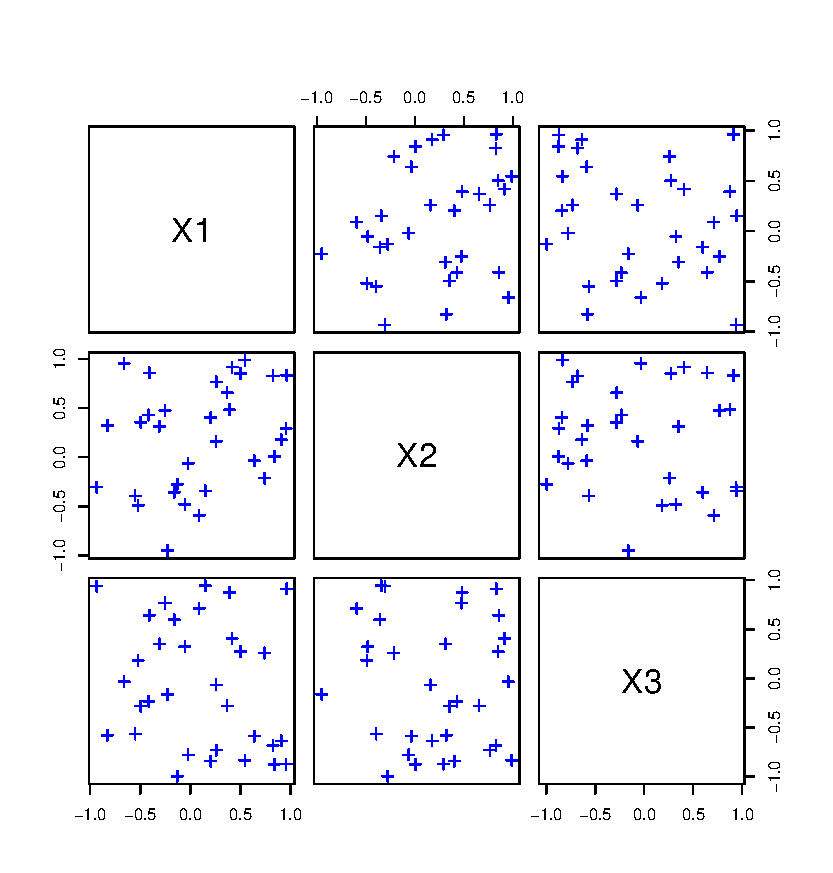
\includegraphics[width=8cm]{Figures/MonteCarlo_DOE.pdf} & 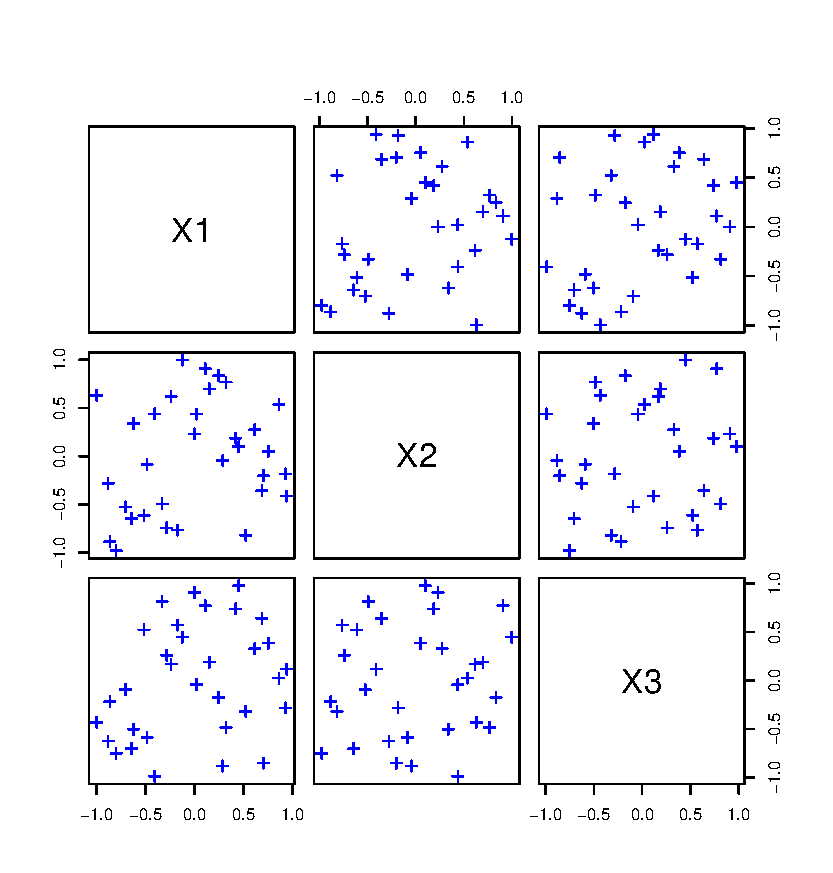
\includegraphics[width=8cm]{Figures/LHS_DOE.pdf}\\
          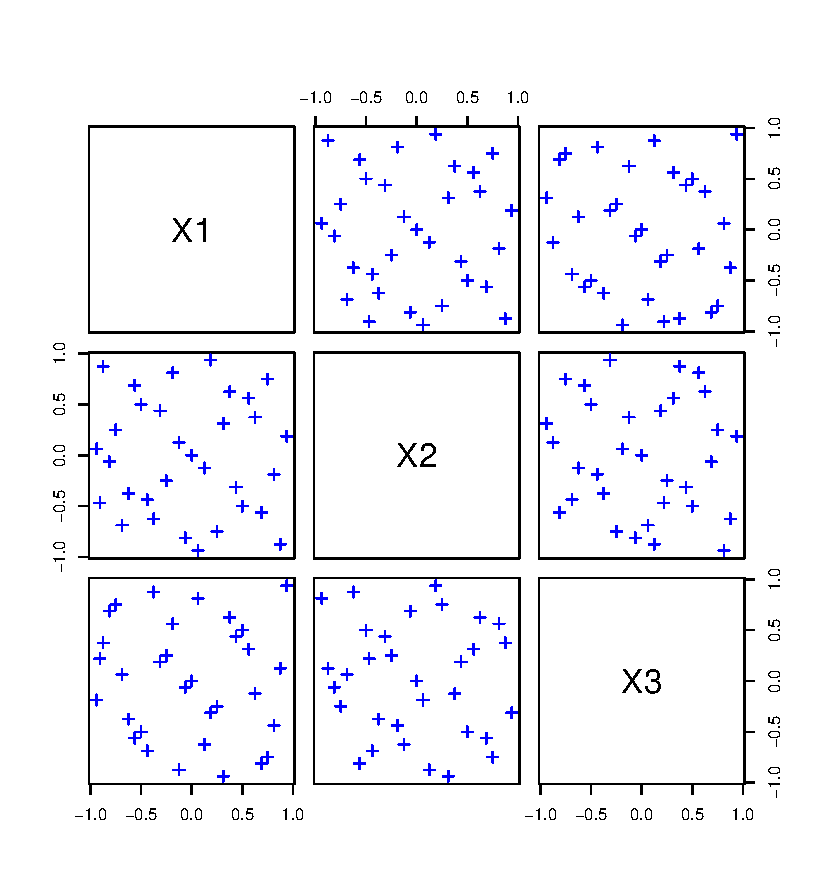
\includegraphics[width=8cm]{Figures/Sobol_DOE.pdf} & 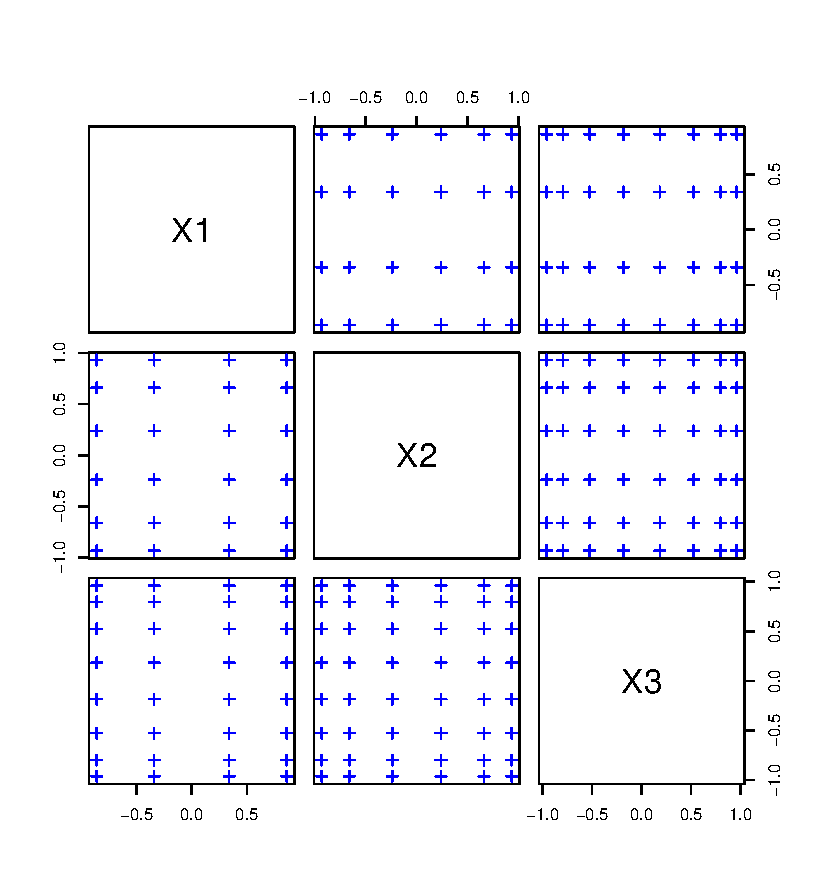
\includegraphics[width=8cm]{Figures/Gauss_DOE.pdf}
        \end{tabular}
      \end{center}

      \vspace*{2mm}

      {\bf Combinatorial generators }\\

      In some situations, one want to explore all the possibilities related to constrained discrete uncertainties. In this case, we need to obtain all the sets of indices fulfilling the constraints. Exemples of constraints are:
      \begin{itemize}
      \item being a subset with $k$ elements of a set with $n$ elements, with $k\leq n$;
      \item being a permutation of $k$ elements taken into a set of $n$ elements, with $k\leq n$;
      \item being an element of a Cartesian product of sets with $n_1,\hdots,n_d$ elements.
      \end{itemize}

      It is important to get indices and not real-valued vectors. The distinction is made explicit by calling these design of experiments \emph{Combinatorial Generators}, which produce collections of indices instead of samples.

      The following figures illustrates the different patterns obtained.
      \newpage
      \begin{center}
        \begin{tabular}{cc}
          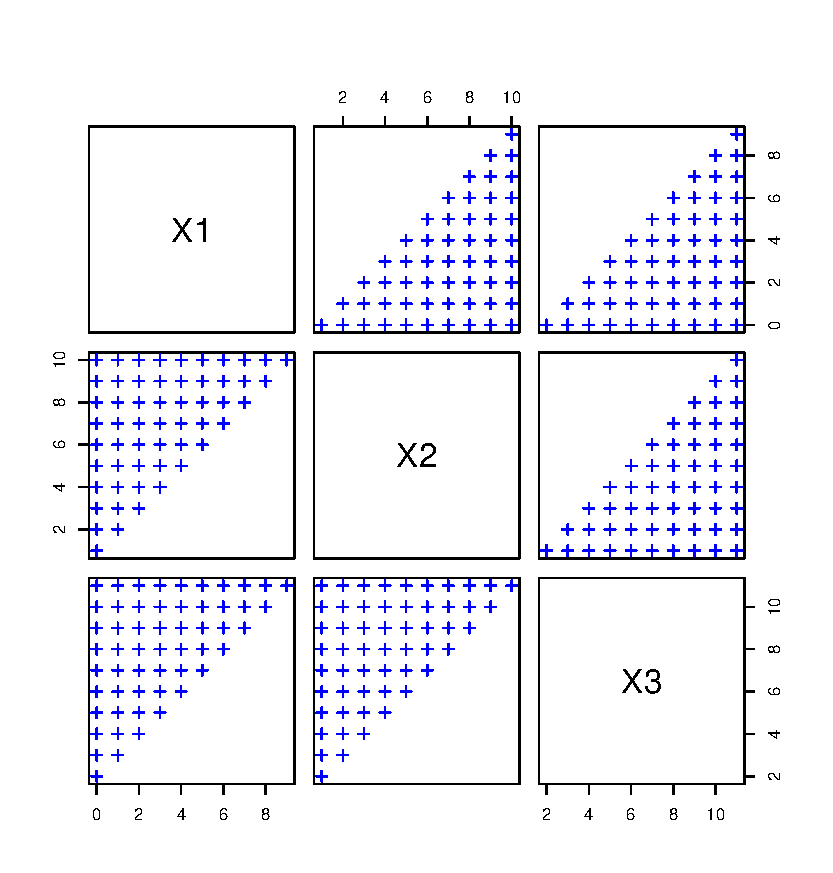
\includegraphics[width=8cm]{Figures/Combinations_DOE.pdf} & 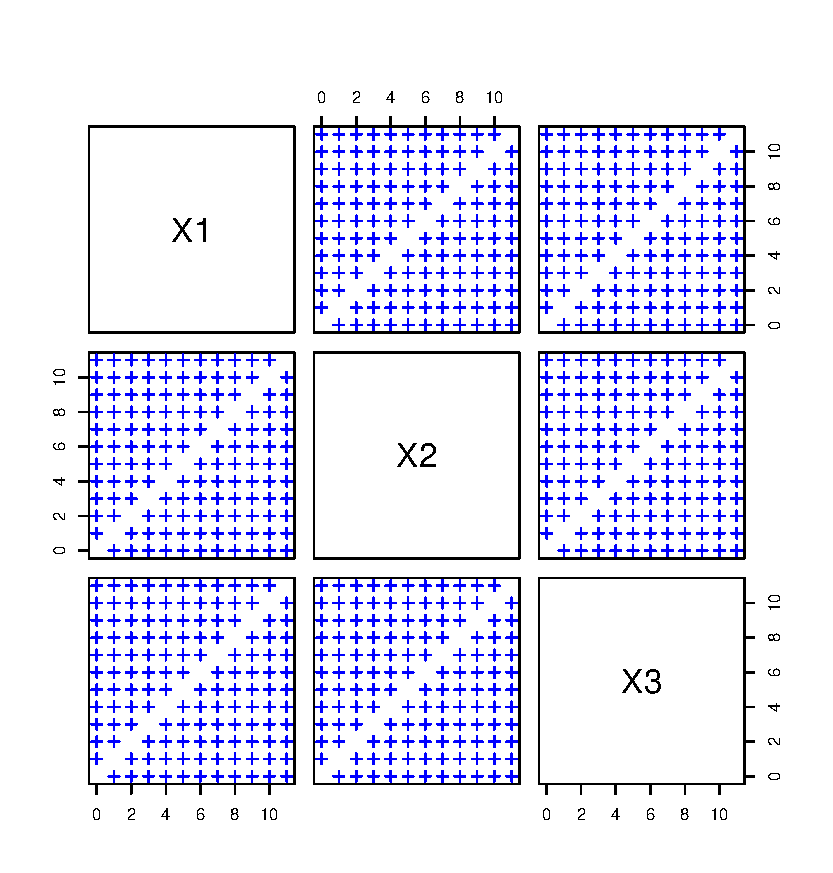
\includegraphics[width=8cm]{Figures/KPermutations_DOE.pdf}\\
          \multicolumn{2}{c}{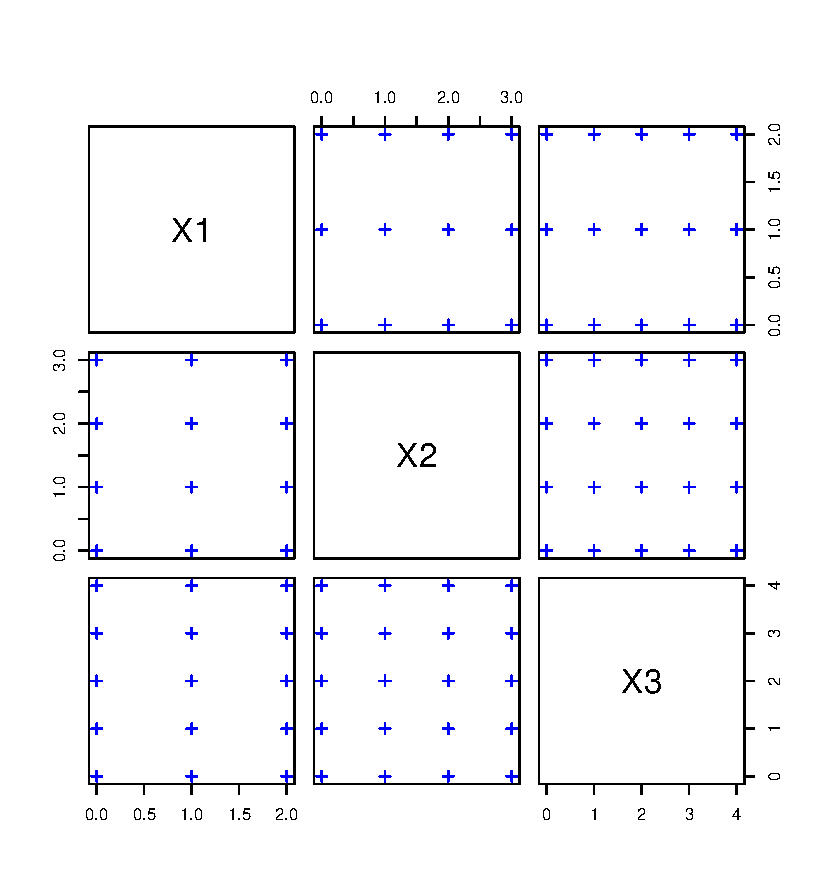
\includegraphics[width=8cm]{Figures/Tuples_DOE.pdf}}
        \end{tabular}
      \end{center}
    }
    {
      --
    }

    \Methodology
        {
          This method is used in step C "Propagation of uncertainty" to evaluate a deterministic minimum-maximum type of criterion for the output value defined in step A "Specifying the Criteria and the Case Study".\\
          It can also be used within the Quasi-Monte carlo technique to approximate the probability of excedding a given threshold.
        }
        {
          --
        }
